\documentclass[a4paper]{article}
\usepackage{graphicx}
\usepackage{float}

\begin{document}

	\title{\Huge{Software Requirement Specification}}
	\author{Group 8 \\ J Lewis	28183488\\
	TGN Machaba	12078027\\
	NS Manana	12064115\\
	JF Maree	28004265\\
	A Volschenk	12054519}
	\maketitle

	\section{Introduction}

		The purpose of this document is to present a detailed description for the mark record and tracking solution. It will explain the purpose and features of the system, what the system will do, as well as the constraints under which it must operate. This document is intended as an official contract between the stakeholders and developers of the system.

	\section{Vision}

		The software solution will be aimed at providing a means for markers in a practical session to record student marks from a mobile device. The purpose is to allow for more efficient marking process, from initial recording of marks to the feedback of results for both lecturer and student. The system should manage recorded marks while ensuring proper authorization to any access of the data it contains. There would be three different user responsibilities, namely: lecturer, marker, and student.
		
		\subsection{Lecturer}
			\begin{itemize}
				\item	Full access to create, read, update and delete data within the lecturer's subject(s).
				\item	Ability to define practical sessions and associate mark allocations to these sessions.
				\item	Ability to open and close the mark inputs for practical sessions.
				\item	Ability to assign markers to practical sessions to enable access to data entry according to a time slot.
				\item	All activity on the system is logged for accountability during auditing.
				\item	Compiling of reports from practical marks.
			\end{itemize}

		\subsection{Marker}
			\begin{itemize}
				\item	Greater efficiency at locating the appropriate student for marking through search functionality.
				\item	Recording marks according to mark sheet set up by lecturer.
				\item	Having a centralized marking environment from which all responsibilities as a marker are accessible.
			\end{itemize}

		\subsection{Student}
			\begin{itemize}
				\item	Faster access to marks progress.
				\item	Ability to view track record and performance.
				\item	Provides accountability of markers involved during mark queries.
			\end{itemize}

	\section{Background}

		Currently the marking process is performed using physical documents. It is required of the marker to obtain a mark sheet from the lecturer, on which the student identification is paired with the results from the practical session. The data is then captured by a third party. This system lacks in accountability and efficiency which can be solved through a software solution and eliminating the need of a third party. The likelihood of marks being lost would also decrease as the data transfer process is diminished from a three step process (marker $\rightarrow$ entry $\rightarrow$ lecturer) to a direct process (marker $\rightarrow$ lecturer). As a result, students would also be able to receive quicker feedback on their work.

		\section{Architectural Requirements}

\subsection{Access Channel Requirements}

\begin{itemize}

\item An android application must be created for marker.
\item This application will be available to the marker at all times.
\item A web interface will be created for the Lecturer and the students
\item The system will access the University's current LDAP system for authentication purposes

\end{itemize}

\subsection{Quality Requirements}

\begin{enumerate}

\item Security:
\begin{itemize}
\item The lecturer will set the privileges of the markers.
\item Fields will are selected will be locked to ensure mutual exclusion.
\item Students will only be able access their own marks.
\item SSL will be used for encryption during data transfer.
\end{itemize}
\item Performance:
\begin{itemize}
\item The system must be able to handle a large number of concurrent users without slowing down response time to anything less than 0.5 seconds.
\end{itemize}
\item Reliability:
\begin{itemize}
\item Software reliability is measured in terms mean time between failures. This consists of mean time to failure and mean time to repair. Reliability between 0 and 1 is good.
\end{itemize}
\item Scalability:
\begin{itemize}
\item The system must be able to handle an increase in the number of departments using it.
\item The system also needs to have increased functionality at low cost.
\end{itemize}
\item Flexibility:
\begin{itemize}
\item The system would need to flexible in the sense that it could be easily adapted to fit new rules and regulations set out to the department or rules set out by a different department.
\end{itemize}
\item Maintainability:
\begin{itemize}
\item The software needs to have measures put in place where errors are easily identifiable and easy to fix. 
\item Unexpected break downs can be traced back to its source.
\item It must be able to cope with a changed environment.
\end{itemize}
\item Audit-ability:
\begin{itemize}
\item A log must be kept, which records everything that happens in the system
\item Lecturers will generate reports from the marks entered
\end{itemize}
\item Integrability:
\begin{itemize}
\item The system must integrate into the system that is already being used by the Department.
\item This involves the use of python, DJANGO and SOAP.
\end{itemize}
\item Usability:
\begin{itemize}
\item First and foremost users must be able to complete the tasks they are allowed to do, otherwise the system is pointless.
\item Any errors caused by the user must be easy to understand and clear.
\item A record of any errors must be kept.
\end{itemize}
\item Cost:
\begin{itemize}
\item The system must be affordable. Nothing more than what is currently in place.
\end{itemize}
\end{enumerate}

\subsection{Integration Requirements}

\begin{itemize}
<<<<<<< HEAD
\item Interface with the current booking system used by the Department.
\item It will use Lightweight Directory Access Protocol along with a SOAP interface.
\item Python and it's DJANGO framework will be used.
\item Databases and servers used by the Department will also need to integrate with the system.
=======

\item Interface with the current booking system used by the Department.
\item It will use Lightweight Directory Access Protocol along with a SOAP interface.
\item Python and it's DJANGO framework will be used.
\item Databases and servers used by the Department will also need to integrate with the system 

>>>>>>> f69a47c25b8dc5780ba91dd15ef54c3944a31604
\end{itemize}


		\subsection{Architecture Constraints}
		
			\subsubsection{Technologies}
		
				\begin{itemize}

					\item{Client interface must run on an Android device}

					\item{Client interface must be accessible through a web browser}
					
					\item{MySQL database must be used to store application data}
					
					\item{Python must be used in order to accommodate existing systems}

				\end{itemize}
				
			\subsubsection{Frameworks}
			
				\begin{itemize}

					\item{The application must be able to interface with the Django framework}

				\end{itemize}

	\section{Functional Requirements}

		\subsection{Introduction}

			This section introduces the functional requirements of the system, as seen by the different stakeholders:

			\subsubsection{Student}
				\begin{flushleft}
				A person who participates in examinable activities, for whom marks are recorded in the system. \linebreak 
				
				Students can:
				\end{flushleft}
				\begin{itemize}

					\item{View Marks}

				\end{itemize}

			\subsubsection{Marker}
				\begin{flushleft}
				A person who is responsible for grading a student, and who has to record marks for all students who he/she has graded. \linebreak 
				
				Markers can:
				\end{flushleft}
				\begin{itemize}

					\item{Input student marks}
					
					\item{View session marks}
					
					\item{Search for student}

				\end{itemize}
				
			\subsubsection{Lecturer}
				\begin{flushleft}
				A person who is responsible for setting examinable activities, as well as the logistics and administration of a particular course. \linebreak 
				
				Lecturers can:
				\end{flushleft}
				\begin{itemize}

					\item{Edit student marks}
					
					\item{View all marks}
					
					\item{Search for student}
					
					\item{Generate reports}
					
					\item{Assign system functions to Markers}
					
					\item{Create and edit marksheets}

				\end{itemize}
			\subsection{Scope and Exclusions}
			\subsubsection{Scope}
			\begin{figure}[h]
				\caption{High Level Use Case Diagram}
<<<<<<< HEAD
				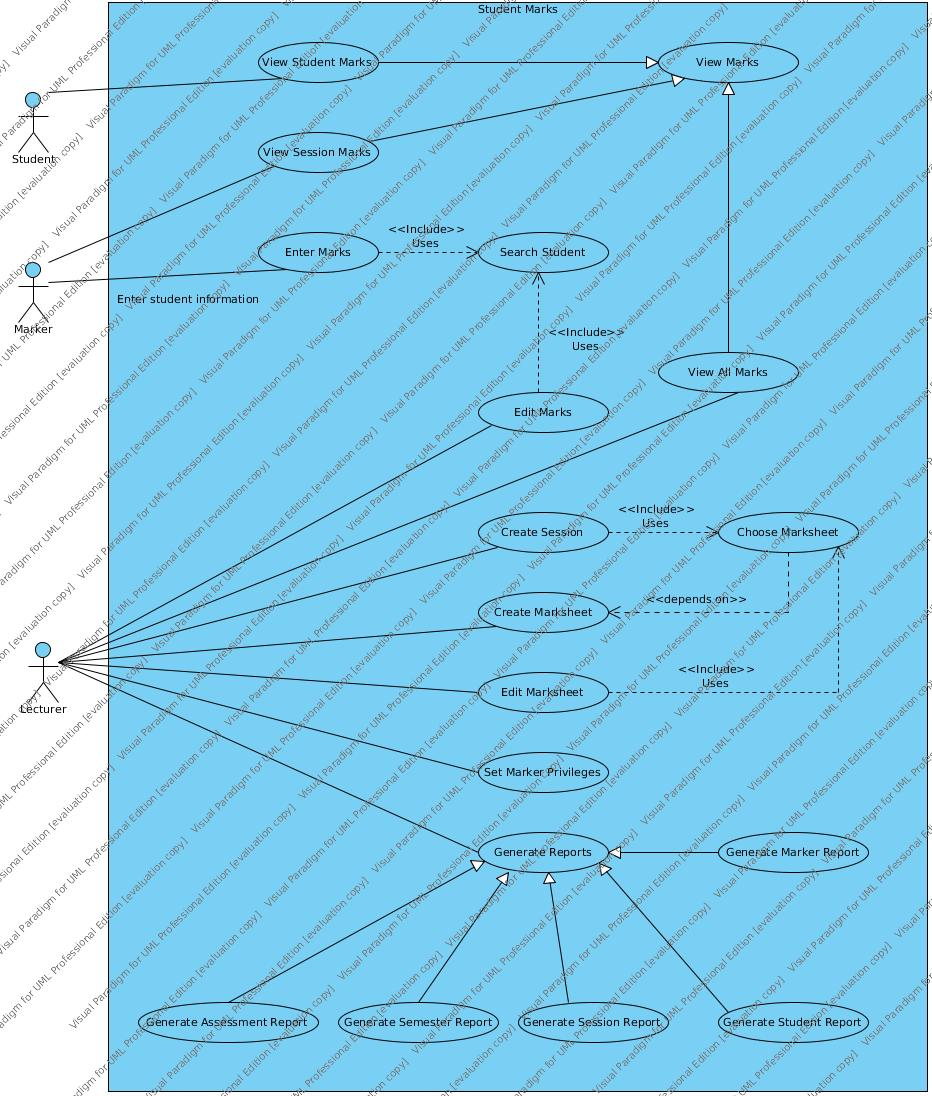
\includegraphics[width=1\textwidth]{StudentMarks}
=======
				%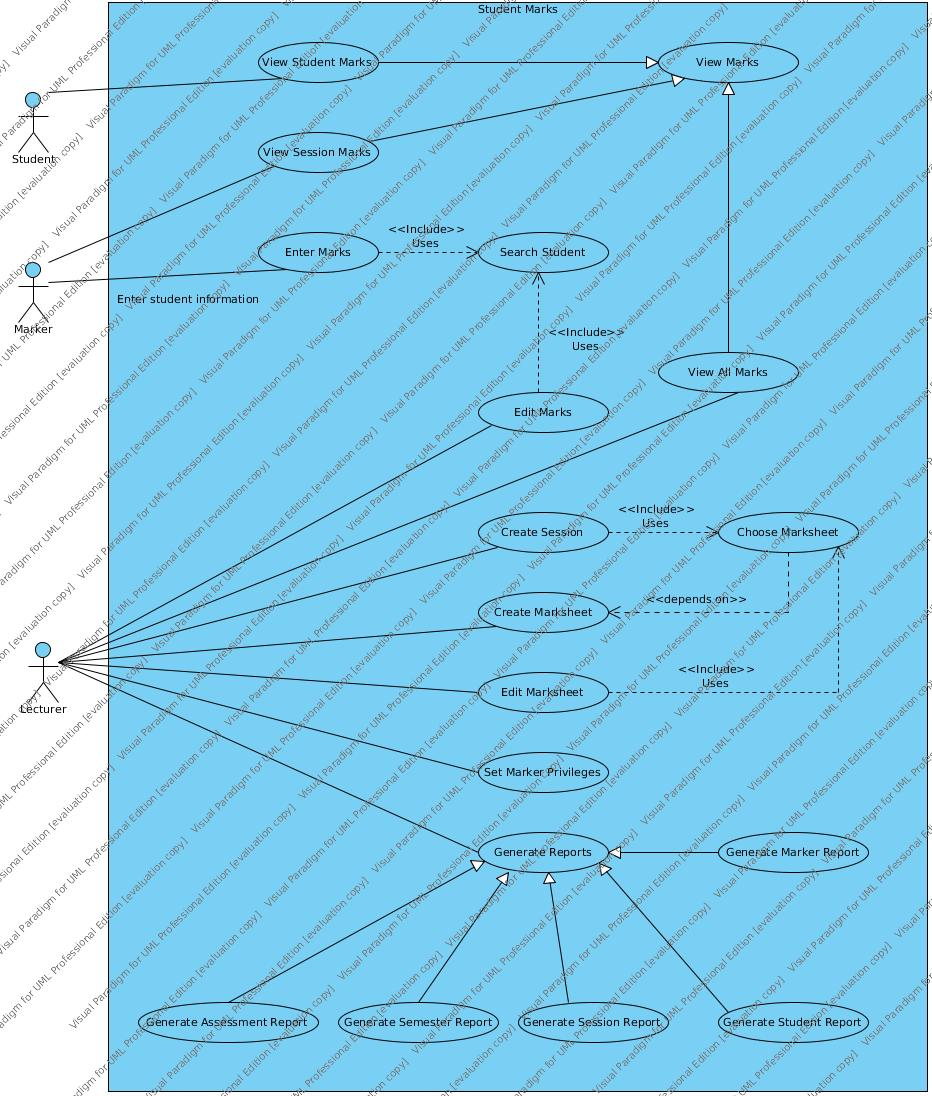
\includegraphics[height=10cm]{StudentMarks}
>>>>>>> siphokazi
			\end{figure}
			\subsubsection{Exclusions}
				\begin{itemize}
				
					\item{The system will not allow registration of Users}
					
					\item{The system will not allow allocation of a Student to a Session (Bookings)}
					
					\item{The system will not allow deletion of any User}
					
					\item{The system will not allow deletion of any Marks}
				
				\end{itemize}

		\subsection{Required Functionality}
		\begin{enumerate}
		\item The system will have a Web and Android application.
		\item The system will have a search panel in which a user types in a student's details (student number/ name/ surname) with auto-complete functionality and displays that will show all possible results of the search.
		\item The system will retrieve the relevant information of a student depending on the access rights said user is granted.
		\item The system shall allow the recording and editing of marks by lecturers and markers.
		\item The system will have a history trail of all edits made to existing marks in the database.
		\item The system aims to provide real-time updates of marks to the database and if this is not possible due to unforseen circumstances, the system will have the option to update information on a smartphone's local storage first.
		\item The system will provide the following security features:
		\begin{itemize}
			\item{Check validity of user attempting to edit before granting access to edit marks.}
			\item{Automatic log off of a user if the system is not in use for more than 15 minutes.}
			\item{Automatic lock after a practical session.}
			\item{Log-in interface to restrict access to the students enrolled, markers and lecturers involved.}
			\item{User authentication checks}
			\item{Students will only be able to view their own marks and no other students' marks when logged in.}
			\item{Markers will only be able to view students in their session}
			\item{Only lecturers and markers will be granted access to enter marks into the database.}
			\item{Only lecturers will obtain a list of all the marks.}
		
		\end{itemize}
		
		\item The system will sanitize the input entered, i.e it will display an error message if the input is invalid.
		\item When entering marks the system will validate if the student is booked for the session.
		\item The system will allow only a lecturer to create a session, assign markers to groups of students and set marker priveleges.
		\item The system will have a reporting functionality that will provide the lecturer with statistics and visual reports such as graphs (distribution, bar), pie charts, average marks, median, mode and standard deviation. 
		\item The system will provide documents in .csv format as exports of marks to lecturers.
		
		\end{enumerate}
			\begin{figure}[H]
				\centering
				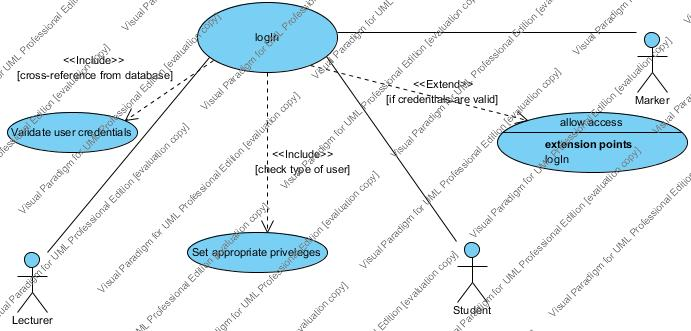
\includegraphics[width=1\textwidth]{logIn}
				\caption{Low Level Use Case Diagrams- Log In}
			\end{figure}
			\begin{figure}[H]
				\centering
				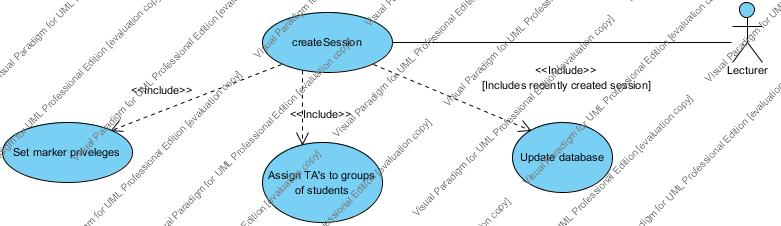
\includegraphics[width=1\textwidth]{createSession}
				\caption{Create Session}
			\end{figure}
			\begin{figure}[H]
				\centering
				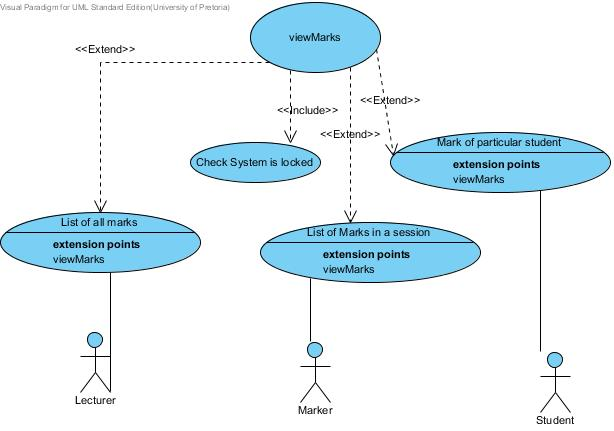
\includegraphics[width=1\textwidth]{viewMarks}
				\caption{View Marks}
			\end{figure}
			\begin{figure}[H]
				\centering
				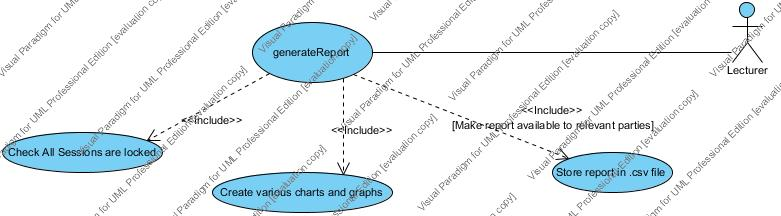
\includegraphics[width=1\textwidth]{generateReport}
				\caption{Generate Report}
			\end{figure}
			\begin{figure}[H]
				\centering
				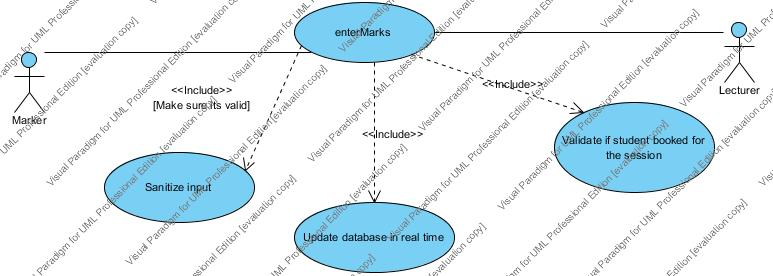
\includegraphics[width=1\textwidth]{enterMarks}
				\caption{Enter Marks}
			\end{figure}
			\begin{figure}[H]
				\centering
				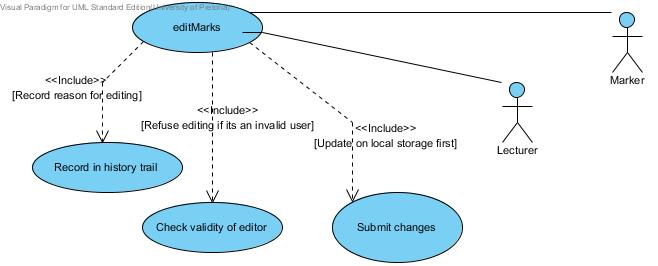
\includegraphics[width=1\textwidth]{editMarks}
				\caption{Edit Marks}
			\end{figure}
			\begin{figure}[H]
				\centering
				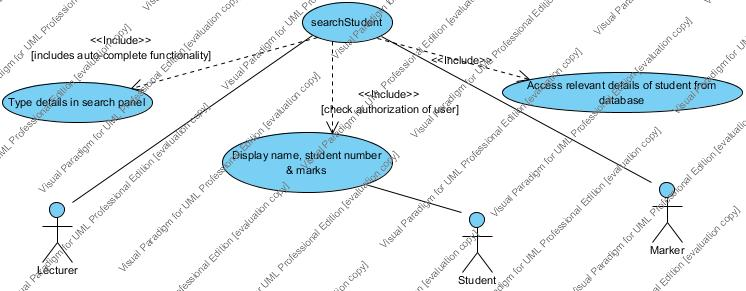
\includegraphics[width=1\textwidth]{searchStudent}
				\caption{Search Student}
			\end{figure}

		\subsection{Use Case Prioritisation}
			\begin{enumerate}
			\item Critical: System is cancelled if functionality is not provided.
			\begin{itemize}
			\item{Lock System - System runs the risk of security breaches if it is not locked.}
			\item{View Marks - The system is rendered useless if users cannot view the marks and details of students whose marks have been entered.}
			\item{Login - Important for access control to prevent unauthorised users entering the system.}
			\item {Set privileges - The system can be susceptible to hacking and corruption of data if this requirement isn't included, which will result in a useless system}
			\item {Create Session - Without this ability the system would not have students to assign to be marked thus rendering the system useless.}
			\item {Edit Marks - Without this functionality the system is susceptible to have incorrect data due to human error that cannot be fixed once entered.}
			\item {Check validity of editor - Once again the system will run the risk of corruption of data if the editor is not authorised to edit the marks.}
			\item {Enter Marks - The marker and lecturer must be able to enter marks otherwise the system is rendered useless.}
			\item {Sanitize input - Invalid input will corrupt the data rendering the system useless.}
			\end{itemize}
			\item Important: System still functional without requirement but client will get less value from it.
			\begin{itemize}
			\item {Search Student - One can still scroll down the list to find a student and the functionality will still remain intact but the system will be less useful.}
			\item { Generate Report - The functionality of recording the marks and storing them in a database is still intact but the system is less useful if you cannot interpret the results}
			\item { Record edits in history trail - This is necessary for accountability if a marker or lecturer changes the marks of students.}
			\end{itemize}
			\item Nice-to-have: Specified requirement but its value is insignificant.
			\begin{itemize}
				\item{Update database in real-time - This isn't a requirement essential for the functioning for the system but it will make the system more efficient}		
			\end{itemize}
			\end{enumerate}
		\subsection{Use Case/Service Contracts}
			
			The following is a list of Pre and Post-Conditions for each use case or service.
			\begin{itemize}
			
				\item 	\textbf{View Student Marks [UC1]}\\*
						\textit{Pre-Conditions:}
								\begin{itemize}
									\item The student must be registered for the module.
									\item The student's session marksheet should be locked.
								\end{itemize}
								
						\textit{Post-Conditions:}
								\begin{itemize}
									\item Marks viewed by a student is added to the Log.
								\end{itemize}
														
				\item	\textbf{View Session Marks [UC2]}\\*
						\textit{Pre-Conditions:}
								\begin{itemize}
									\item The marker must be the designated marker for the session.
								\end{itemize}
								
						\textit{Post-Conditions:}
								\begin{itemize}
									\item Marks viewed by the marker is added to the Log.
								\end{itemize}
														
				\item	\textbf{Enter Marks[UC3]}\\*
						\textit{Pre-Conditions:}
								\begin{itemize}
									\item The marker must be the designated marker for the session.
									\item The student being marked must be registered for the session.
									\item The session should be open and not locked.
								\end{itemize}
								
						\textit{Post-Conditions:}
								\begin{itemize}
									\item The students's marks are in the database.
									\item The student's Marks have been entered is added to the Log.
								\end{itemize}
														
				\item	\textbf{Edit Marks[UC4]}\\*
						\textit{Pre-Conditions:}
								\begin{itemize}
									\item The Lecturer must be a Lecturer for the module.
								\end{itemize}
								
						\textit{Post-Conditions:}
								\begin{itemize}
									\item The new marks are in the databse.
									\item The mark changes are added to the Log.
								\end{itemize}
														
				\item	\textbf{Search Student[UC5]}\\*
						\textit{Pre-Conditions:}
								\begin{itemize}
									\item The student must be registered for the module or session.
								\end{itemize}
								
						\textit{Post-Conditions:}
								\begin{itemize}
									\item None
								\end{itemize}
														
				\item	\textbf{Set Marker Privileges[UC6]}\\*
						\textit{Pre-Conditions:}
								\begin{itemize}
									\item The lecturer must be a Lecturer for the module.
									\item The marker must be designated to the module as a marker.
								\end{itemize}
								
						\textit{Post-Conditions:}
								\begin{itemize}
									\item The marker's privileges are set in the databse.
									\item The marker's Privilege changes are added to the Log.
								\end{itemize}
														
				\item	\textbf{Generate Reports[UC7]}\\*
						\textit{Pre-Conditions:}
								\begin{itemize}
									\item The Lecturer must be a Lecturer for the module.
									\item The sessions should all be locked.
								\end{itemize}
								
						\textit{Post-Conditions:}
								\begin{itemize}
									\item None
								\end{itemize}
														
				\item	\textbf{Create Marksheet[UC8]}\\*
						\textit{Pre-Conditions:}
								\begin{itemize}
									\item The Lecturer must be a Lecturer for the module.
									\item The marksheet should not already exist.
								\end{itemize}
								
						\textit{Post-Conditions:}
								\begin{itemize}
									\item The new Marksheet is created.
									\item The Marksheet creation is added to the Log.
								\end{itemize}
														
				\item	\textbf{Edit Marksheet[UC9]}\\*
						\textit{Pre-Conditions:}
								\begin{itemize}
									\item The Lecturer must be a Lecturer for the module.
									\item The marksheet should already exist.
								\end{itemize}
								
						\textit{Post-Conditions:}
								\begin{itemize}
									\item The Changes are saved to the marksheet.
									\item The Marksheet was edited is added to the Log.
								\end{itemize}
														
				\item	\textbf{Create Session[UC10]}\\*
						\textit{Pre-Conditions:}
								\begin{itemize}
									\item The Lecturer must be a Lecturer for the module.
									\item The session should not already exist.
								\end{itemize}
								
						\textit{Post-Conditions:}
								\begin{itemize}
									\item A new session is created.
									\item The session creation is added to the Log.
								\end{itemize}
														
				\item	\textbf{Assign Marker to group[UC11]}\\*
						\textit{Pre-Conditions:}
								\begin{itemize}
									\item The Lecturer must be a Lecturer for the module.
									\item The Marker must be a designated marker for the module.
								\end{itemize}
								
						\textit{Post-Conditions:}
								\begin{itemize}
									\item The marker is designated to a group.
									\item The marker's assignment to group is added to the Log.
								\end{itemize}
														
				\item	\textbf{Login[UC12]}\\*
						\textit{Pre-Conditions:}
								\begin{itemize}
									\item The user must be a valid user with valid credentials.
									\item The user should not already be logged in.
								\end{itemize}
								
						\textit{Post-Conditions:}
								\begin{itemize}
									\item Privileges are set for the user's current session.
									\item The user's Login time is added to the Log.
								\end{itemize}
														
				\item	\textbf{View all marks[UC13]}\\*
						\textit{Pre-Conditions:}
								\begin{itemize}
									\item The Lecturer must be a Lecturer for the module.
									\item The sessions should all be locked.
								\end{itemize}
								
						\textit{Post-Conditions:}
								\begin{itemize}
									\item None
								\end{itemize}
			\end{itemize}

		\subsection{Process Specification}

		\subsection{Domain Objects}
		
			\subsubsection{Class Diagram}
			
			\begin{figure}[h]
				\caption{Class Diagram}
				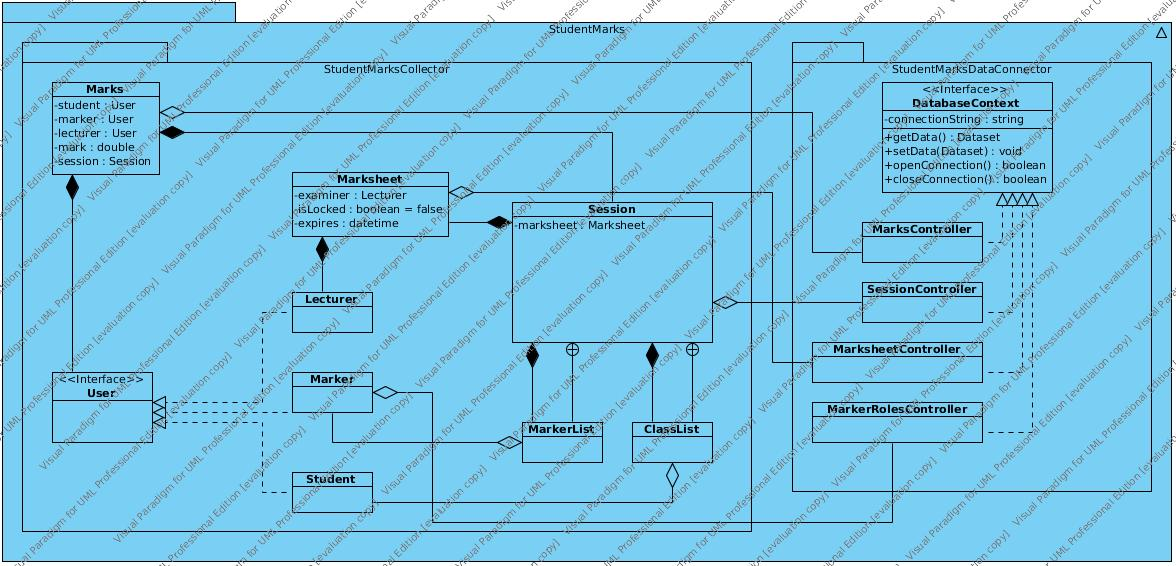
\includegraphics[width=1\textwidth]{StudentMarksClassDiagram}
			\end{figure}

	\section{Open Issues}

	\section{Glossary}
		
		\begin{itemize}
			\item UC* - Use Case number * (where '*' represents a number)
			\item Pre-Condition - A condition that must be satisfied Before the given service or use case.
			\item Post-Condition - A condition that must be satisfied After the given service or use case.
		\end{itemize}

\end{document}
